\section{Earth Centered Inertial} \label{sec:icrf} 
The standard Earth centered inertial frame is the ICRF, defined in 1995 with locations given for 22 quasars and other bright radio objects. This definition was extended by the addition of more sources in 2000. See the IERS memo \cite{IERS2003} for further information. The ICRF is the best-determined and most stable reference frame at the epoch year 2000. The ICRS is almost identical to the inertial frame known as J2000.

\textbf{Coordinate Frame: } Non-Rotating Inertial

\begin{itemize}
\item X-axis: Defined as the cross product of the Z-axis (as defined below) and the Earth mean orbit pole of J2000 (i.e. the ecliptic pole of J2000). The X-axis of this coordinate frame is the Earth vernal equinox of J2000.
\item Y-axis: Completes a standard, right-handed coordinate frame.
\item Z-axis: Defined as the pole vector of the Earth Mean Equator of J2000
(where J2000 = Julian date 2451545.0 ).
\end{itemize}
For the difference between ICRF and the older J2000 systems, see the JEOD \hyperTLD.


\begin{figure}[htp]
\centering
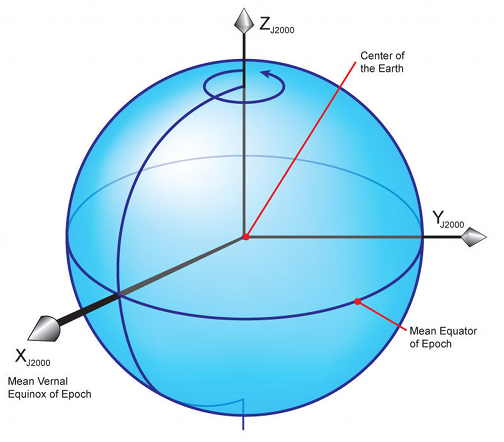
\includegraphics [width=7in]{figs/fig4.png}
\caption{International Celestial Reference Frame}
\label{fig:4}
\end{figure}

\subsection{Example Earth ICRF }
To set up a non-spherical Earth one must invoke a transformation from inertial to body fixed coordinates must be set up. As an example,set up a sim\_object in the S\_define file, for instance see SIM 2 in the \hyperTutorial. Set the coordinate system the S\_define sim object Earth must contain the following parameters, see the \hyperTutorial\ for all variable and parameter definitions:

\begin{verbatim}

// SIM_OBJECT: earth
// This sim object models the space environment.
//=============================================================================
sim_object {

   //
   // Data structures
   //
   environment/planet:  Planet               planet
      (environment/planet/data/earth.d);


   environment/gravity:    SphericalHarmonicsGravityBody   gravity_body
      (environment/gravity/data/earth_GGM02C.d);

   environment/RNP/RNPJ2000:        RNPJ2000             rnp
      (environment/RNP/RNPJ2000/data/rnp_j2000.d);

   environment/RNP/RNPJ2000:        NutationJ2000Init    nut_init
      (environment/RNP/RNPJ2000/data/nutation_j2000.d);

   environment/RNP/RNPJ2000:        PolarMotionJ2000Init pm_init 
      (environment/RNP/RNPJ2000/data/polar_motion/xpyp_daily.d);
      
   //
   // Initialization jobs
   //
   P_ENV (initialization) environment/gravity:
   earth.gravity_body.initialize_body ( );

   P_ENV (initialization) environment/gravity:
   env.gravity.add_grav_source(
      Inout GravityBody & grav_body = earth.gravity_body );

   P_ENV (initialization) environment/planet:
   earth.planet.register_model(
      Inout GravityBody & grav_body   = earth.gravity_body,
      Inout DynManager  & dyn_manager = dynamics.manager );
 
   P_ENV (initialization) environment/RNP/RNPJ2000:
   earth.rnp.initialize(
      Inout DynManager & manager = dynamics.manager );
   
   P_ENV (initialization) environment/RNP/GenericRNP:
   earth.rnp.nutation->initialize(
      In PlanetRotationInit * init = &earth.nut_init );
 
   P_ENV (initialization) environment/RNP/GenericRNP:
   earth.rnp.polar_motion->initialize(
      In PlanetRotationInit * init = &earth.pm_init );

   P_ENV (initialization) environment/RNP/RNPJ2000:
   earth.rnp.update_rnp (
      In TimeTT & time_tt = time.tt,
      In TimeGMST & time_gmst = time.gmst,
      In TimeUT1 & time_ut1 = time.ut1 ); 
   
   P_BODY (initialization) environment/planet:
   earth.planet.initialize( );

   //
   // Environment class jobs
   //
   
   (LOW_RATE_ENV, environment) environment/RNP/RNPJ2000:
   earth.rnp.update_rnp (
      In TimeTT & time_tt = time.tt,
      In TimeGMST & time_gmst = time.gmst,
      In TimeUT1 & time_ut1 = time.ut1 );
   //
   // Derivative class jobs
   //
   P_ENV Idynamics (derivative) environment/RNP/RNPJ2000:
   earth.rnp.update_axial_rotation(
      In TimeGMST & time_gmst = time.gmst );

} earth;
\end{verbatim}
This also contains the propagation of a spacecraft in Earth orbit.
An example of the inertial coordinates are given in input.py file found in the SET\_test/RUN\_4 directory of Tutorial SIM\_4.


